\documentclass[12pt,a4paper]{article}
\usepackage[utf8]{inputenc}
\usepackage[russian]{babel}
\usepackage[OT1]{fontenc}
\usepackage{mathtools}
\usepackage{amsfonts}
\usepackage{amssymb}
\usepackage{enumitem}
\usepackage{alltt}
\usepackage{graphicx}
\usepackage{indentfirst}
\usepackage{caption}
\usepackage{float}
\usepackage{wrapfig}
\setlength{\parindent}{0.75cm}
\graphicspath{{pictures/}}
\DeclareGraphicsExtensions{.png}
\usepackage[left=15mm,right=15mm,top=2cm,bottom=2cm]{geometry}
\author{Глотов Алексей}
\begin{document}
\newpage
\begin{center}
\footnotesize{{ГОСУДАРСТВЕННОЕ АВТОНОМНОЕ ОБРАЗОВАТЕЛЬНОЕ УЧРЕЖДЕНИЕ}\break
{ВЫСШЕГО ОБРАЗОВАНИЯ}
\break
{\bf {МОСКОВСКИЙ ФИЗИКО-ТЕХНИЧЕСКИЙ ИНСТИТУТ}}
\break
\small{(НАЦИОНАЛЬНЫЙ ИССЛЕДОВАТЕЛЬСКИЙ УНИВЕРСИТЕТ)}}
\break
\hfill \break
\hfill \break
\begin{center}
\normalsize{Кафедра общей физики}
\end{center}
\hfill \break
\hfill \break
\hfill \break
\hfill \break

\begin{center}
\normalsize {Лабораторная работа 1.3.3}
\end{center}
\hfill \break\\
\large{\textbf{Измерение вязкости воздуха по течению в тонких трубках}}
\end{center}
\begin{flushleft}
\hfill \break
\hfill \break
\hfill \break
\hfill \break
\hfill \break
\hfill \break
\hfill \break
\hfill \break
\hfill \break
\hfill \break
\hangindent=9cm
\normalsize{Преподаватель:}\hfill
\normalsize{доцент Игуманов А.Ю.}\\
\hfill \break
\normalsize{Обучающийся:}\hfill
\normalsize{Глотов А.А} \\
\hfill \break
\end{flushleft}
\hfill \break
\hfill \break
\hfill \break
\hfill \break
\hfill \break
\hfill \break
\hfill \break
\hfill \break
\hfill \break
\hfill \break
\hfill \break

\begin{center}
Долгопрудный \break
 2022
\end{center}
\thispagestyle{empty}
\newpage
\begin{center}
\large{\bf Введение} 
\end{center}
\begin{center}
\large{Аннотация}
\end{center}
\par Данная работа посвящена изучению воздуха по прямой трубе тонкого сечения. Используются следующие методы измерений: анализ графиков зависимости Q($\Delta$P), а также линеаризированных графиков зависимостей Q(R). Расход газа измеряется с помощью газового счётчика и секундомера, перепад давления в трубке - с помощью микроманометра.
\par Цели работы: экспериментально исследовать свойства течения газов по тонким трубкам при различных числах Рейнольдса; выявить область применимости закона Пуазейля и с его помощью определить коэффициент вязкости воздуха
\hfill \break
\begin{center}
\large{Приборы и материалы}
\end{center}
\begin{itemize}
\item Система подачи воздуха(компрессор, подводящие трубки)
\item Набор трубок различного диаметра с выводами для подсоединения микроманометра
\item Секундомер: $\Delta_{\text{сек}}$=0.4c (удвоенное среднее время реакции человека)
\item Газовый счетчик ГСБ-400 \hfill \break
Устройство
\begin{enumerate}
\item Измерительная шкала (1 оборот = 5 л)
\item Счётно-суммирующее устройство (1 ед. = 1 л)
\item Индикатор горизонтального уровня
\item Водомерное устройство
\item Трубка для подачи газа
\item Трубка для отвода газа
\item Патрубки для подключения
внешнего манометра
\item Место установки термометра
\item Регулируемые ножки
\item Сливное отверстие
\end{enumerate}
\begin{figure}[H]
\centering
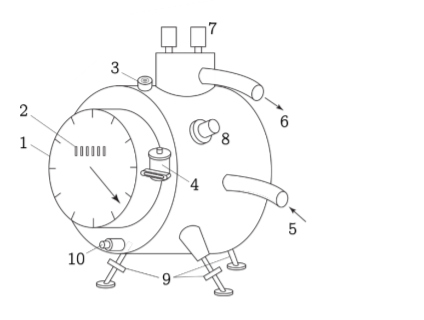
\includegraphics[width=9cm, height=7cm]{1.3.3_1}
\caption{Схема газового счетчика}
\label{pic:1}
\end{figure}
Характеристики
\begin{itemize}
\item Класс точности: 1,0
\item Пределы измерения расхода: от 20 л/ч до 1000 л/ч
\item Цена наименьшего деления: 0,02 л
\item Предел измерения стрелочного механизма (1 оборот): 5 л
\item Максимально допустимый перепад давления: 600 мм вод. ст. (5885 Па)
\end{itemize}
\item Спиртовой микроманометр MMH-2400
Устройство
\begin{enumerate}
\item Сосуд с рабочей жидкостью
\item Измерительная шкала
\item Стойка для регулировки наклона K
\item Место крепления измерительных
трубок («–» и «+»)
\item Переключатель режима работы
(металлический рычажок):
(0) — установка нуля;
(+) — проведение измерений.
\item Поплавок регулировки уровня спирта (для установки нуля)
\item Винт, регулирующий глубину погружения поплавка
\item Индикаторы горизонтального уровня
\item Регулируемые ножки
\end{enumerate}
\begin{itemize}
\item Класс точности: 1,0
\item Рабочая жидкость: спирт этиловый ректификованный 96%
 (плотность 0,8095±0,0005 г/см3 при 20℃)
\end{itemize}
\end{itemize}
\begin{figure}[H]
\centering
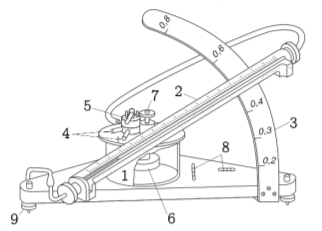
\includegraphics[width=10cm, height=6cm]{1.3.3_2}
\caption{Схема микроманометра}
\label{pic:1}
\end{figure}
\newpage
\begin{center}
\large{Экспериментальная установка}
\end{center}
\begin{figure}[H]
\centering
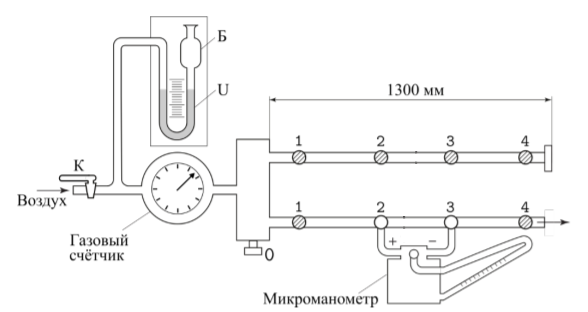
\includegraphics[width=10cm, height=6cm]{1.3.3_3}
\caption{Схема экспериментальной установки}
\label{pic:2}
\end{figure}
\par Поток воздуха под давлением, превышающим атмосферное, поступает через газовый счётчик в тонкие металлические трубки под действием компрессора, интенсивность подачи регулируется краном К. Трубки снабжены съёмными заглушками на концах и рядом миллиметровых отверстий, к которым можно подключать микроманометр. В рабочем состоянии открыта заглушка на рабочей трубке, микроманометр подключен к ее двум выводам, а остальные отверстия плотно закрыты.
\par Перед входом установлен водяной U-образный манометр. При превышении максимального избыточного давления на входе счётчика (~30 см.вод.ст) вода выплескивается в баллон Б.
\begin{center}
\large{Теоретические сведения}
\end{center}
$\eta$ - вязкость среды \hfill \break
Q - объемный расход газа; Q зависит от перепада давления $\Delta$P, плотности $\rho$ и вязкости $\eta$ газа, от радиуса трубы R и её длины l(исследуемой части)
\par Характер течения в трубе может быть ламинарным либо турбулентным. При ламинарном течении линии тока не смешиваются, скорости вдоль них одинаковы. При турбулентном образовываются вихри, перемешиваются слои течения газа, линии тока; постоянной является только средняя скорость течения газа.
\par Характер течения определяется числом Рейнольдса:
\begin{equation}
Re=\frac{\rho{ua}}{\eta}
\end{equation}
$\rho$ - плотность среды, u - характерная скорость потока, a - характерный размер системы (для тонкой трубы - радиус R). С ростом Re может быть достигнуто число $Re_{\text{кр}}$, при котором характер течения нельзя считать ламинарным. 
\par В условиях данной работы используются следующие данные и приближения: $Re_{\text{кр}} \approx 10^3$, $\eta \approx 2*10^{-5}$ газ несжимаемый ($\rho$ = const), перепад давления мал, а число Маха значительно меньше 1
\par При ламинарном течении объёмый расход газа описывается формулой Пуазейля:
\begin{equation}
Q = \frac{\pi{R^4}}{8l\eta}\Delta{P}
\end{equation}
$\Delta{P}$ - разность давлений в выбранных сечениях, расстояние между которыми равно l. Необходимо отметить, что формула(1) работает при Re < 1000, т.е. течение ламинарно с запасом. Для выполнения формулы (2) необходимо, чтобы удельный объём газа существенно не изменялся, т.е. перепад давления должен быть малым по сравнению с внешним (атмосферным) давлением. 
\par Необходимо также отметить, что стационарное течение устанавливается не сразу, а на какой то определенной длине, которое приблизительно можно посчитать по формуле
\begin{equation}
l_{\text{уст}}=0.2*R*Re
\end{equation} 
0.2 - экспериментально установленное значение, справедливое для данной работы. Если $l_{\text{уст}}<l$, то течение нельзя считать установившимся, а значит и ламинарным.
\par Рассмотрим турбулентное течение газа в тонкой трубке. В простейшей модели: предположим, что при больших значениях Re ($Re \gg Re_{\text{кр}}$) можно считать практически идеальной, так что параметры её течения не зависят от коэффициента вязкости. Отсюда получаем:
\begin{equation}
Q=const*R^{5/2}\sqrt{\frac{\Delta{P}}{\rho{l}}}
\end{equation}
\newpage
\begin{center}
\large {\bf Результаты измерений и обработка данных}\break
\end{center}
1) Согласно паспорту приборов (газового счётчика и микроманометра) их погрешности составляют $\Delta_{V} = 0,2\text{л}=0.2\text{дм}^{3}$ для счётчика и 1 деление для микроманометра (конкретное значение давления зависит от набора данных) \hfill \break
2) Проверим работоспособность установки, пронаблюдаем качественно изменения показаний газового счётчика и микроманометра при изменении степени открытия крана. \hfill \break
3) $T_{\text{ср}}=22,6\pm0.1^{\circ}C$ - температура окружающей среды \hfill\break
$\mu=0.92$ - влажность воздуха \hfill \break
$p_{a}=10^5\text{Па}$ - атмосферное давление
\par Запишем диаметры трубок: \hfill \break
$d_{1}=3.95\pm0.05\text{мм}$ \hfill \break
$d_{2}=3.00\pm0.01\text{мм}$ \hfill \break
$d_{3}=5.30\pm0.05\text{мм}$ \hfill \break
Тогда значение плотности воздуха можно считать приблизительно равным : $\rho = 1.18\frac{\text{кг}}{\text{м}^3}$ \hfill \break
4) Отметим, что Q связана с u - характерной скоростью потока - следующим соотношением: $Q=\pi{R^2}$. Тогда из (1) получим, что:
\begin{equation}
Q_{\text{кр}}=\frac{Re_{\text{кр}}\eta\pi{R}}{\rho}
\end{equation}
\par Теперь по формуле Пуазейля (2) возможно рассчитать $\Delta{P}_{\text{кр}}$   \hfill \break
\begin{center}
\begin{tabular}{|c|c|c|c|c|}
\hline 
№ трубки & $Q_{\text{кр}}$, $\frac{\text{дм}^3}{c}$ & l, \text{м} & $\Delta{P}$, Па & $l_{\text{уст}}$, м \\ 
\hline 
1 & 0,105 & 0.9 & 316,8 & 0,395 \\ 
\hline 
2 & 0,080 & 0.415 & 333,5 & 0,3 \\ 
\hline 
3 & 0,141 & 0.9 & 131,1 & 0,53 \\ 
\hline 
\end{tabular} 
\end{center}
Таким образом, можно сделать вывод, что каждой из трёх длин достаточно для того, чтобы считать течение на этих участках установившимся \hfill \break
5) Пронаблюдаем за изменением перепада давления с изменением положения крана. Заметим (приблизительно) переход с ламинарного на турбулентное течение. \hfill \break
Для первой трубки искомое давление составило 292,20 Па; для второй - 319,47 Па; для третьей - 138,31 Па \hfill \break
Таким образом, можно сказать, что теоретические данный совпадают с полученными на практике \hfill \break
6)$Q=\frac{\Delta{V}}{\Delta{t}}\Rightarrow\varepsilon_{Q}=\frac{\sigma_{V}}{\Delta{V}}+\frac{\sigma_{t}}{\Delta{t}}$ \hfill \break
Таким образом, относительная погрешность измерения расхода складывается из относительных погрешностей времени и объёма. Для необходимой оценки условимся, что каждая из них не должна превышать значения 0,5$\%$. Тогда: \hfill \break
$V_{min}=\frac{\sigma_{V}}{0.005}=4\text{л}$, $t_{min}=\frac{\sigma_{t}}{0.005}=80c$ \hfill \break 
Отметим также, что т.к. некоторые измерения занимают довольно продолжительное время, в них без потери точности можно использовать меньший временной промежуток. 
\newpage
7)Измерения на 1 трубке 
\begin{center}
\begin{tabular}{|c|c|c|c|c|c|}
\hline 
N, \text{дел} & $\Delta{V}, \text{дм}^3$ & $\Delta{t}$,с  & Q, $\frac{\text{м}^3}{c}$ & $\Delta{P}$, \text{Па} & $\frac{\Delta{P}}{l}, \frac{\text{Па}}{с}$ \\ 
\hline 
8 & 3.00 & 251.5 & 1.19 & 31.17 & 34.63 \\ 
\hline 
15 & 2.50 & 118.7 & 2.11 & 58.44 & 64.93 \\ 
\hline 
20 & 3.00 & 107.3 & 2.80 & 77.92 & 86.58 \\ 
\hline 
30 & 4.00 & 101.0 & 3.96 & 116.88 & 129.86 \\ 
\hline 
38 & 5.00 & 97.7 & 5.12 & 148.05 & 164.50 \\ 
\hline 
45 & 5.00 & 82.5 & 6.06 & 175.32 & 194.80 \\ 
\hline 
54 & 5.00 & 69.9 & 7.15 & 210.38 & 233.76 \\ 
\hline 
60 & 5.00 & 62.3 & 8.03 & 233.76 & 259.73 \\ 
\hline 
68 & 5.00 & 56.3 & 8.89 & 264.93 & 294.37 \\ 
\hline 
75 & 5.00 & 52.3 & 9.56 & 292.20 & 324.67 \\ 
\hline 
84 & 5.00 & 49.5 & 10.1 & 327.26 & 363.62 \\ 
\hline 
95 & 5.00 & 47.7 & 10.5 & 370.12 & 411.24 \\ 
\hline 
106 & 5.00 & 46.5 & 10.8 & 412.98 & 458.87 \\ 
\hline 
120 & 5.00 & 44.9 & 11.1 & 467.52 & 519.47 \\ 
\hline 
142 & 5.00 & 42.4 & 11.8 & 553.23 & 614.70 \\ 
\hline 
\end{tabular}
\end{center} \hfill \break
$\Delta{P}=9.8067*0.9932*K*N$, где 9,8067 - ускорение свободного падения - и 0,9932 - коэффициент, зависящий от условий окружающей среды - коэффициенты перевода показаний на шкале манометра в давление \hfill \break
K=0.4 - коэффициент чувствительности микроманометра \hfill \break
Аналогично проведем эксперимент на 2 и 3 трубках и занесем значения в таблицы (K=0.8 и 0.2 соответственно) \hfill \break
\begin{center}
\begin{tabular}{|c|c|c|c|c|c|}
\hline 
N, \text{дел} & V, $\text{дм}^3$ & $\Delta{t}$, c & Q, $\frac{\text{м}^3}{c}*10^{-5}$ & $\Delta{P}$, Па & $\frac{\Delta{P}}{l}$ \\ 
\hline 
7 & 3.0 & 129.5 & 2.32 & 54.54 & 131.42 \\ 
\hline 
14 & 3.0 & 65.9 & 4.55 & 109.09 & 262.87 \\ 
\hline 
20 & 5.0 & 83.8 & 5.97 & 155.84 & 375.52 \\ 
\hline 
25 & 5.0 & 72.9 & 6.86 & 194.80 & 469.40 \\ 
\hline 
30 & 5.0 & 64.4 & 7.76 & 233.76 & 563.28 \\ 
\hline 
34 & 5.0 & 60.0 & 8.33 & 264.93 & 638.39 \\ 
\hline 
41 & 5.0 & 54.5 & 9.17 & 319.47 & 769.81 \\ 
\hline 
44 & 5.0 & 53.4 & 9.36 & 342.85 & 826.14 \\ 
\hline 
\end{tabular}
\end{center} \hfill \break
\begin{center}
\begin{tabular}{|c|c|c|c|c|c|}
\hline 
N, \text{дел} & V,$\text{дм}^3$ & $\Delta{t}$, c & Q, $\frac{\text{м}^3}{c}*10^{-5}$ & $\Delta{P}$, \text{Па} & $\frac{\Delta{P}}{l}, \frac{\text{Па}}{м}$ \\ 
\hline 
16 & 4,0 & 96,1 & 4,16 & 31,17 & 34,63 \\ 
\hline 
20 & 5,0 & 49,8 & 10,04 & 38,96 & 43,29 \\ 
\hline 
28 & 5,0 & 72,7 & 6,88 & 54,54 & 60,60 \\ 
\hline 
37 & 5,0 & 57,4 & 8,71 & 72,08 & 80,09 \\ 
\hline 
46 & 5,0 & 46,5 & 10,75 & 89,61 & 99,57 \\ 
\hline 
58 & 5,0 & 39,2 & 12,76 & 112,98 & 125,53 \\ 
\hline 
71 & 5,0 & 34,9 & 14,33 & 138,31 & 153,68 \\ 
\hline 
80 & 4,0 & 27,0 & 14,81 & 155,84 & 173,16 \\ 
\hline 
93 & 4,0 & 26,2 & 15,27 & 181,16 & 201,29 \\ 
\hline 
104 & 4,0 & 25,6 & 15,63 & 202,59 & 225,10 \\ 
\hline 
117 & 5,0 & 30,5 & 16,39 & 227,92 & 253,24 \\ 
\hline 
129 & 5,0 & 29,3 & 17,06 & 251,29 & 279,21 \\ 
\hline 
144 & 5,0 & 28,3 & 17,67 & 280,51 & 311,68 \\ 
\hline 
\end{tabular} 
\end{center} 
8) 
\begin{center}
\begin{tabular}{|c|c|c|c|c|c|c|c|c|c|c|}
\hline 
\multicolumn{11}{|c|}{1 трубка} \\ 
\hline 
l, \text{м} & 0,112 & 0,412 & 0,812 & 1,312 & 0,300 & 0,700 & 1,200 & 0,400 & 0,900 & 0,500 \\ 
\hline 
N, \text{дел} & 63 & 114 & 132 & 259 & 53 & 124 & 197 & 72 & 145 & 75 \\ 
\hline 
$\Delta{P}$, \text{Па} & 122,72 & 222,07 & 257.14 & 504,53 & 103,24 & 241,55 & 383,76 & 140,26 & 282,46 & 146,10 \\ 
\hline 
\multicolumn{11}{|c|}{2 трубка} \\ 
\hline 
l, \text{м} & 0,115 & 0,415 & 0,615 & 0,20 & 0,500 & 0,300 & - & - & - & - \\ 
\hline 
N, \text{дел} & 62 & 64 & 145 & 38 & 82 & 33 & - & - & - & - \\ 
\hline 
$\Delta{P}$, \text{Па} & 120,78 & 124,67 & 282,46 & 74,02 & 159,74 & 64,28 & - & - & - & - \\ 
\hline 
\multicolumn{11}{|c|}{3 трубка} \\ 
\hline 
l, \text{м} & 0,115 & 0,415 & 0,815 & 1,315 & 0,300 & 0,700 & 1,200 & 0,400 & 0,900 & 0,500 \\ 
\hline 
N, \text{дел} & 24 & 40 & 59 & 81 & 18 & 37 & 57 & 20 & 44 & 24 \\ 
\hline 
$\Delta{P}$, \text{Па} & 46,75 & 77,92 & 114,93 & 157,79 & 35,06 & 72,08 & 111,04 & 38,96 & 85,71 & 46,75 \\ 
\hline 
\end{tabular} 
\end{center}
При расчёте $\Delta{P}$ K=0.2 \hfill \break
10) Согласно полученным экспериментальным точкам, ламинарность потока на всех трубках обеспечивается при значении градиента давления $\frac{\Delta{P}}{l}=125\frac{\text{Па}}{\text{м}}$
Максимальный достижимый градиент давления, обеспечивающий турбулентность течения равен 857$\frac{\text{Па}}{\text{м}}$
Соответственные значения расхода газа: $3,75*10^{-5}, 1,44*10^{-5} \text{ и } 12.77*10^{-5} \frac{\text{м}^3}{c}$ для ламинарного течения; $15.89*10^{-5}, 9.36*10^{-5} \text{ и } 32.59*10^{-5} \frac{\text{м}^3}{c}$ - для турбулентного \hfill \break
11)Построим графики зависимостей Q($\Delta{P}$)
\begin{figure}[H]
\centering
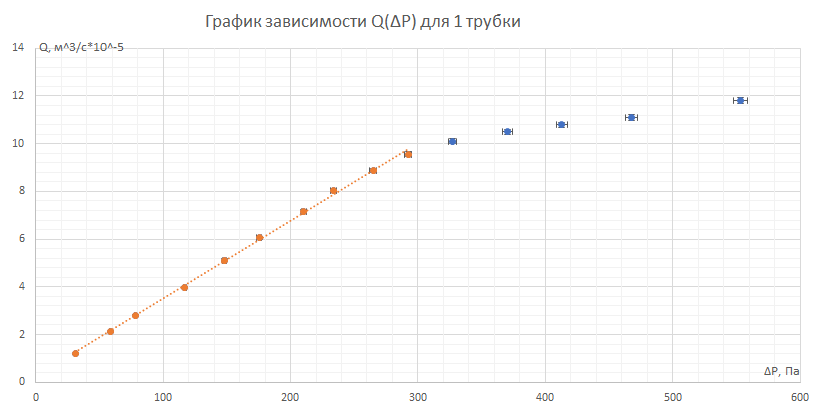
\includegraphics[width=14cm, height=7cm]{1.3.3_gr_1}
\end{figure}
\begin{figure}[H]
\centering
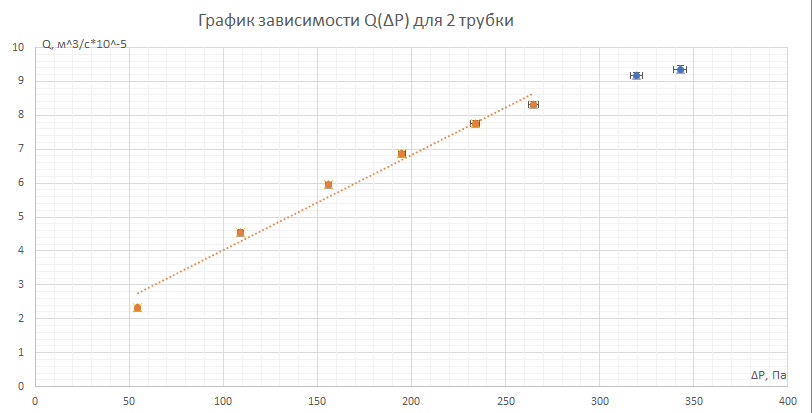
\includegraphics[width=14cm, height=7cm]{1.3.3_gr_2}
\end{figure}
\begin{figure}[H]
\centering
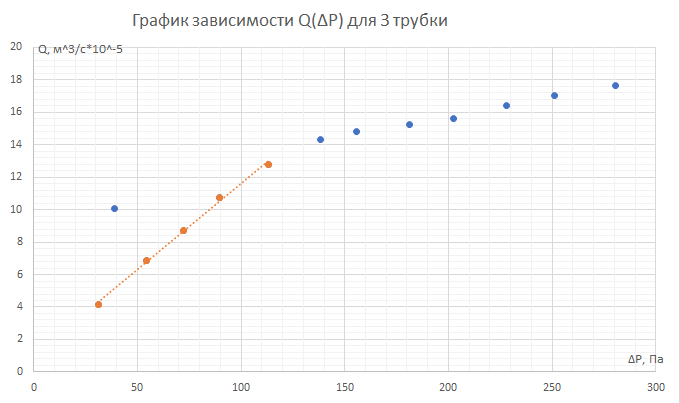
\includegraphics[width=14cm, height=7cm]{1.3.3_gr_3}
\end{figure}
Оранжевым цветом выделены точки, для которых течение газа можно считать ламинарным. 
\par Таким образом, $\Delta{P}_{\text{кр}}$ можно считать равным $(310 \pm 20)$ Па для первой трубки, $(290 \pm 30)$ Па - для второй и $(125 \pm 15)$ Па - для третьей, что подтверждается теоретическими расчётами. Соответственные им $Q_{\text{кр}}$ равны $(9.8 \pm 0.3)*10^{-5} \frac{\text{м}^3}{c}$, $(8.8 \pm 0.4)*10^{-5} \frac{\text{м}^3}{c}$ и $(13.5 \pm 0.8)*10^{-5} \frac{\text{м}^3}{c}$ 
\par Определим угловые коэффициенты для линейных участков наших графиков. \hfill \break
$\alpha=\frac{<Q\Delta{P}>-<\Delta{P}><Q>}{<Q^2>-<Q>^2}$ \;\;\;\;\;\;\; $\sigma_{\alpha}=\sqrt{\frac{1}{N-2}(\frac{<{Q}^2>-<Q>^2}{<{\Delta{P}}^2>-<\Delta{P}>^2}-{\alpha}^2)}$ \hfill \break
$\alpha_{1}=3.27*10^{-7}\frac{\text{м}^3}{\text{Па*с}}$  \;\;\;\;\;\;\;\;\; $\sigma_{\alpha_{1}}=0.04*10^{-7}\frac{\text{м}^3}{\text{Па*с}}$  \hfill \break
$\alpha_{2}=2.8*10^{-7}\frac{\text{м}^3}{\text{Па*с}}$ \;\;\;\;\;\;\;\;\;\; $\sigma_{\alpha_{2}}=0.2*10^{-7}\frac{\text{м}^3}{\text{Па*с}}$ \hfill \break
$\alpha_{3}=1.06*10^{-6}\frac{\text{м}^3}{\text{Па*с}}$ \;\;\;\;\;\;\;\;\; $\sigma_{\alpha_{2}}=0.05*10^{-6}\frac{\text{м}^3}{\text{Па*с}}$ \hfill \break
$\alpha=\frac{\pi{R^4}}{8l\eta}\Rightarrow\eta=\frac{\pi{R^4}}{8l\alpha}$\hfill \break
$\sigma_{\eta}=\sqrt{(\sigma^{\text{случ}}_{\eta})^2+(\sigma^{\text{приб}}_{\eta})^2}$ \hfill \break
$\sigma^{\text{приб}}_{\eta}=\eta(\frac{\sigma_{R}}{R}+\frac{\sigma_{l}}{l})$\;\;\;\;\;\;\;\;\;\; $\sigma^{\text{случ}}_{\eta}=\eta\frac{\sigma_{\alpha}}{\alpha}$ \hfill \break
$\eta_{1}=2,0*10^{-5}\frac{\text{кг}}{\text{м*с}}$ \;\;\;\;\;\;\;\;\;\; $\sigma_{\eta_{1}}=0.1*10^{-5}\frac{\text{кг}}{\text{м*с}}$ \hfill \break
$\eta_{2}=1,7*10^{-5}\frac{\text{кг}}{\text{м*с}}$ \;\;\;\;\;\;\;\;\;\; $\sigma_{\eta_{2}}=0.1*10^{-5}\frac{\text{кг}}{\text{м*с}}$ \hfill \break
$\eta_{3}=2,0*10^{-5}\frac{\text{кг}}{\text{м*с}}$ \;\;\;\;\;\;\;\;\;\; $\sigma_{\eta_{3}}=0.1*10^{-5}\frac{\text{кг}}{\text{м*с}}$
\par Из формулы (5) выразим значение $Re_{\text{кр}}$: $Re_{\text{кр}}=\frac{Q_{\text{кр}}\rho}{\eta\pi{R}}$ \hfill \break
$\sigma_{Re}=Re(\frac{\sigma_{Q_{\text{кр}}}}{Q_{\text{кр}}}+\frac{\sigma_{\eta}}{\eta}+\frac{\sigma_{R}}{R})$ \hfill \break
$(Re_{\text{кр}})_{1}=(930 \pm 90)$ \hfill \break
$(Re_{\text{кр}})_{2}=(1300 \pm 140)$ \hfill \break
$(Re_{\text{кр}})_{3}=(960 \pm 110)$ \hfill \break
12) Построим графики зависимости $\Delta{P}(x)$
\begin{figure}[H]
\centering
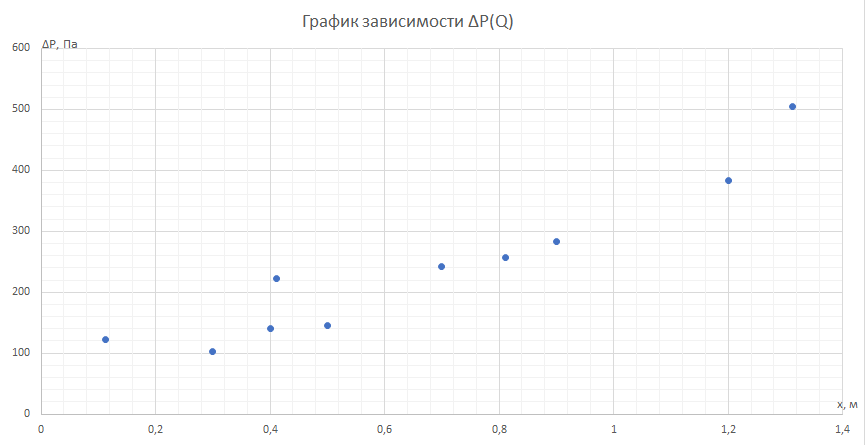
\includegraphics[width=14cm, height=7cm]{1.3.3_gr_4}
\end{figure}
\begin{figure}[H]
\centering
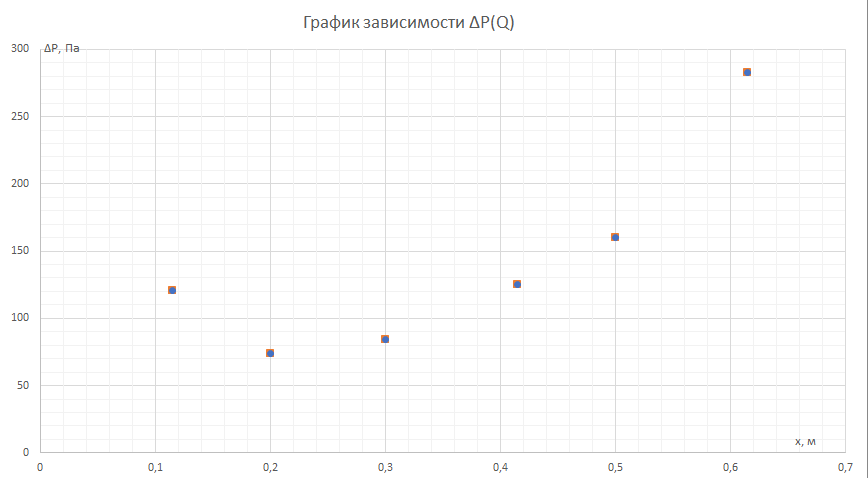
\includegraphics[width=14cm, height=7cm]{1.3.3_gr_5}
\end{figure}
\begin{figure}[H]
\centering
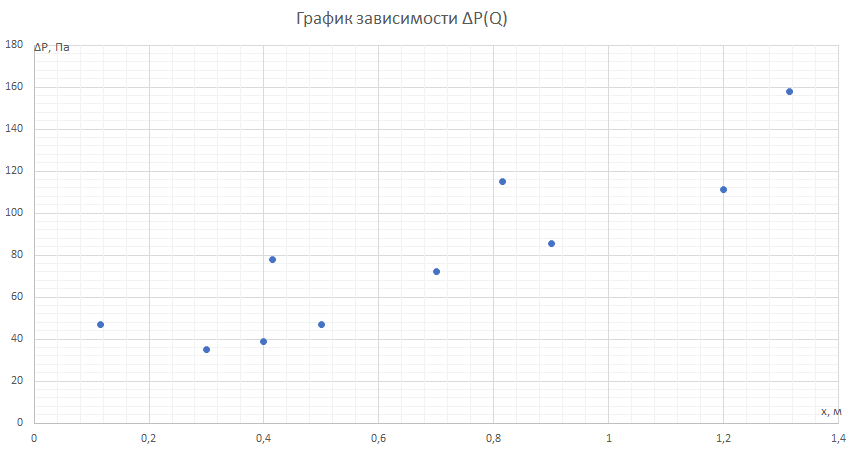
\includegraphics[width=14cm, height=7cm]{1.3.3_gr_6}
\end{figure}
\par Из графиков можно сделать вывод, что устоявшимся движение можно считать приблизительно на 0,3м, 0,2м и 0,3м, что заметно меньше, чем расчетные показатель. \hfill \break
13)По точкам, полученным в п.10 построим графики ln(Q)(ln(R))
\begin{figure}[H]
\centering
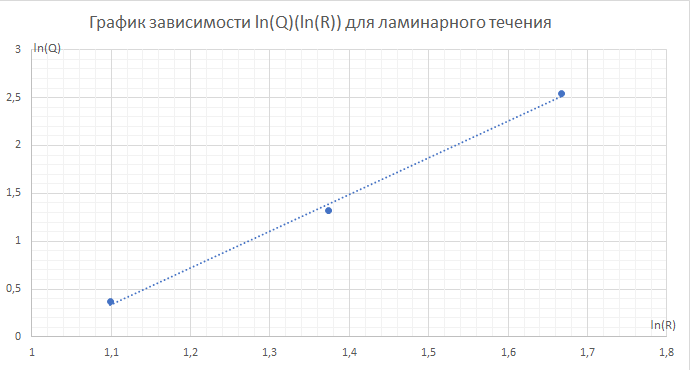
\includegraphics[width=14cm, height=7cm]{1.3.3_gr_7}
\end{figure}
\begin{figure}[H]
\centering
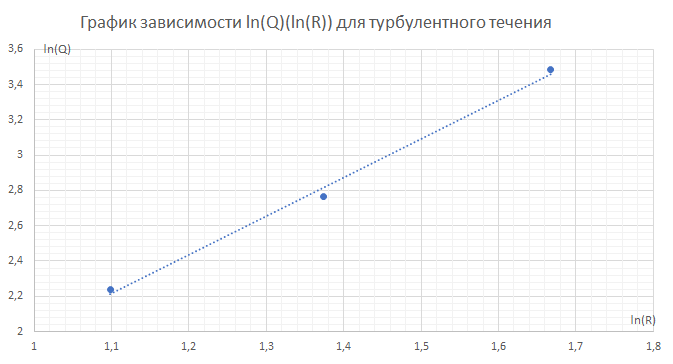
\includegraphics[width=14cm, height=7cm]{1.3.3_gr_8}
\end{figure}
Посчитав коэффициенты наших графиков, получим значения угловых коэффициентов 3,84 и 2,20. Таким образом, можно считать подтвержденной теоретическую модель, описывающую исследуемую зависимость.
\newpage
\begin{center}
\large Обсуждение результатов и выводы
\end{center}
\par В ходе работы был исследован ряд зависимостей величин, характеризующих течение газа в тонкой трубе круглого сечения как друг от друга, так и от различных параметров трубки. При анализе полученных экспериментальных данных было установлено, что формула Пуазейля действительно справедлива в реальных условиях, проверены и доказаны характеры зависимостей объёмного расхода газа (Q) от радиуса трубок (R). Доказано, что действительно существует ламинарное и турбулентные течения и замечен переходный период, когда движение уже точно не является ламинарным, но и однозначно не определяется как турбулентное.
\par При анализе результатов были получены значения вязкости воздуха и чисел Рейнольдса для каждой из трёх исследуемых трубок. Установлено, что вязкость действительно не зависит от радиуса тонкой трубы круглого сечения и равна $(2,0\pm 0,1)*10^{-5}\frac{\text{кг}}{\text{м*с}}$, что совпадает с табличными при наших условиях (1,9).
\par С хорошей точностью (не более 6\%) были получены значения для вязкости газа. Наибольший вклад внесла случайная погрешность, что говорит о необходимости увеличения количества измерений с целью ее уменьшения, а также, желательно, увеличения точности приборов. Из-за несовершенства измерительных приборов из анализа были вынужденно исключены значения, полученные со второй трубки, т.к. невозможно получить данные выше определенного предела, а также достаточно высокой погрешности измерений. Не возможно достоверно оценить погрешность полученного числа Рейнольдса, т.к. необходимые значения были получены "на глаз" из графика, что говорит о необходимости увеличения количества измерений и точности измерительный приборов, чтобы была возможность точно установить момент смены характера течения. 
\end{document}